\chapter{Regression for Numeric Prediction}
\label{chap:regression}
\chapterguide
  {You should understand relationships, sampling uncertainty, and the difference between exploration and validation.}
  {fit a multiple linear regression, interpret coefficients cautiously, evaluate predictions on held-out data, and diagnose residual errors.}

\section{Regression predicts a numeric target}
In supervised learning, the dataset includes an outcome to be predicted. \term{Regression} is used when that target is numeric, such as price, demand, temperature, or concentration.

A multiple linear model has the form
\[
\hat{y}=\beta_0 + \beta_1x_1 + \cdots + \beta_px_p.
\]
The coefficients describe modelled changes in the prediction while holding the other included features fixed. That is not automatically a causal effect.


\section{What a fitted line is minimising}
Ordinary least squares chooses coefficients to minimise the sum of squared residuals. In a one-feature model, each residual is the vertical difference between the observed target and the fitted line.

\begin{utpfig}[Regression geometry and residuals]{The vertical segments are residuals. Squaring them makes large errors contribute disproportionately to the least-squares objective.}{fig:regression-geometry}
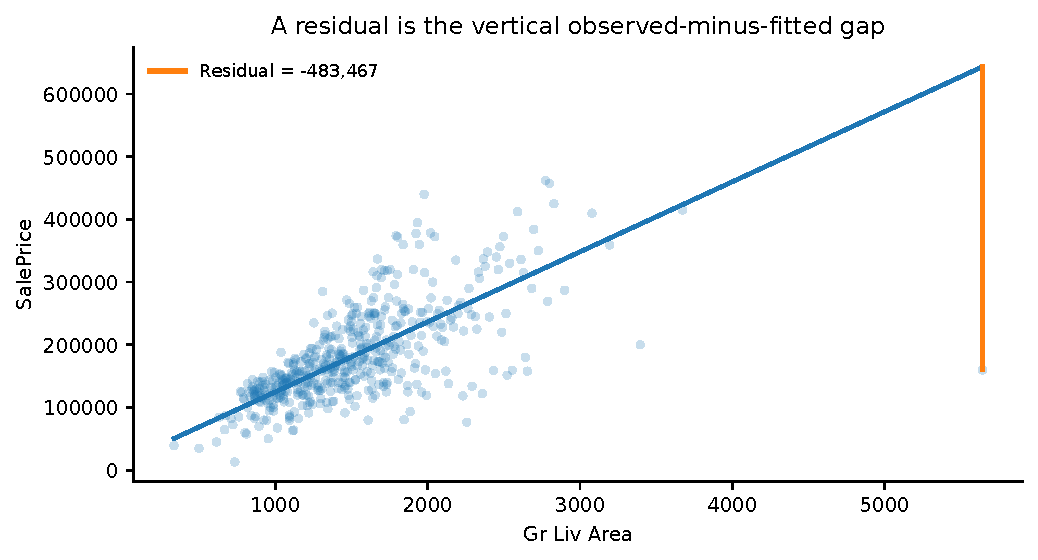
\includegraphics[width=0.80\linewidth]{figures_generated/regression_residual_geometry.pdf}
\end{utpfig}

In multiple regression, the geometry lives in higher-dimensional feature space, but the interpretation is similar: predictions are linear combinations of the included features and residuals measure unexplained target variation.


\section{Training error is not enough}
A flexible model can fit patterns specific to the observed sample. To evaluate generalisation, split the data so some observations are not used to fit the model.

\begin{utpfig}[Train/test workflow]{Model parameters are learned from the training set. The test set is touched only after the model and preprocessing choices are fixed.}{fig:train-test-regression}
\begin{tikzpicture}[x=\linewidth,y=1cm,
  card/.style={draw=UTPBlue!65,fill=UTPPaleBlue,rounded corners=1.8mm,
    line width=0.7pt,text width=0.27\linewidth,
    minimum width=0.34\linewidth,minimum height=1.18cm,
    inner xsep=4mm,inner ysep=2mm,align=center,
    font=\scriptsize\color{UTPNavy}},
  flow/.style={-{Stealth[length=2.2mm,width=1.6mm]},
    line width=0.9pt,draw=UTPTeal},
  testflow/.style={-{Stealth[length=2.2mm,width=1.6mm]},
    line width=0.9pt,draw=UTPOrange!85!black},
  targetflow/.style={-{Stealth[length=2.2mm,width=1.6mm]},
    line width=0.8pt,draw=UTPOrange!85!black,dashed},
  flowlabel/.style={fill=white,rounded corners=1mm,
    inner xsep=2.5mm,inner ysep=1mm,
    font=\tiny\bfseries}]
\node[card,draw=UTPTeal!80,fill=UTPPaleTeal] (all) at (0.50,4.20)
  {\textcolor{UTPTeal}{\textbf{01  AVAILABLE DATA}}\\[4pt]
   Features and target\\before splitting};
\node[card] (train) at (0.28,0.85)
  {\textcolor{UTPBlue}{\textbf{02A  TRAINING PARTITION}}\\[4pt]
   Used to learn\\model parameters};
\node[card,draw=UTPOrange!80,fill=UTPPaleOrange] (test) at (0.72,0.85)
  {\textcolor{UTPOrange!85!black}{\textbf{02B  TEST PARTITION}}\\[4pt]
   Held out from\\model fitting};
\node[card] (model) at (0.28,-1.15)
  {\textcolor{UTPBlue}{\textbf{03A  FIT + FREEZE}}\\[4pt]
   Model and preprocessing\\are now fixed};
\node[card,draw=UTPOrange!80,fill=UTPPaleOrange] (features) at (0.72,-1.15)
  {\textcolor{UTPOrange!85!black}{\textbf{03B  TEST FEATURES}}\\[4pt]
   Apply frozen\\preprocessing only};
\node[card,draw=UTPTeal!80,fill=UTPPaleTeal] (pred) at (0.50,-3.15)
  {\textcolor{UTPTeal}{\textbf{04  TEST PREDICTIONS}}\\[4pt]
   Fixed model applied\\to test features};
\node[card,draw=UTPTeal!80,fill=UTPPaleTeal] (eval) at (0.50,-5.05)
  {\textcolor{UTPTeal}{\textbf{05  EVALUATE}}\\[4pt]
   MAE, RMSE, and\\residual diagnostics};
\coordinate (branch) at (0.50,2.45);
\draw[draw=UTPTeal,line width=0.9pt] (all.south) -- (branch);
\fill[UTPTeal] (branch) circle (1.2pt);
\node[flowlabel,text=UTPTeal] at (0.50,2.95)
  {TRAIN / TEST SPLIT};
\draw[flow] (branch) -| (train.north);
\draw[testflow] (branch) -| (test.north);
\draw[flow] (train.south) -- (model.north);
\draw[testflow] (test.south) -- (features.north);
\coordinate (merge) at (0.50,-2.15);
\draw[draw=UTPTeal,line width=0.9pt] (model.south) |- (merge);
\draw[draw=UTPOrange!85!black,line width=0.9pt] (features.south) |- (merge);
\fill[UTPTeal] (merge) circle (1.15pt);
\draw[flow] (merge) -- (pred.north);
\draw[flow] (pred.south) -- (eval.north);
\draw[targetflow] (test.east) -- ++(0.09\linewidth,0) |- (eval.east);
\node[flowlabel,text=UTPOrange!85!black] at (0.82,-4.78)
  {HELD-OUT TARGETS};
\end{tikzpicture}
\end{utpfig}


\section{Coefficient interpretation is conditional}
In a multiple linear model, $\beta_j$ describes the fitted change in the prediction associated with a one-unit increase in $x_j$ while the other included features are held fixed. This is a model-based conditional association. If features are strongly correlated, ``holding all others fixed'' may describe combinations that are rare in the data and coefficients can become unstable.

Categorical variables are represented through indicator variables relative to a reference group. Interactions allow the effect of one feature to change depending on another feature, which makes the fitted relationship more flexible but also changes how main coefficients should be interpreted.


\section{Error metrics answer different questions}
For residuals \(e_i=y_i-\hat{y}_i\):
\[
MAE=\frac{1}{n}\sum|e_i|,
\qquad
RMSE=\sqrt{\frac{1}{n}\sum e_i^2}.
\]
MAE is an average absolute miss in target units. RMSE penalises large misses more strongly. \(R^2\) compares squared error with a mean-only baseline but should not replace error in meaningful units.

\begin{dstable}
\begin{tabularx}{\linewidth}{@{}D{1.8cm}YD{5.8cm}@{}}
\toprule
\rowcolor{DSPaleBlue!92}
\textbf{Metric} & \textbf{Useful interpretation} & \textbf{Limitation} \\
\midrule
MAE & typical absolute error & treats all misses linearly \\
RMSE & emphasises large errors & sensitive to extreme errors \\
\(R^2\) & fraction of baseline variance explained & less direct operational meaning \\
\bottomrule
\end{tabularx}
\end{dstable}


\begin{utpfig}[Observed versus predicted on held-out data]{Perfect predictions would fall on the dashed 45-degree line. Distance from that line is prediction error; systematic deviations suggest bias in some part of the target range.}{fig:regression-pred-actual}
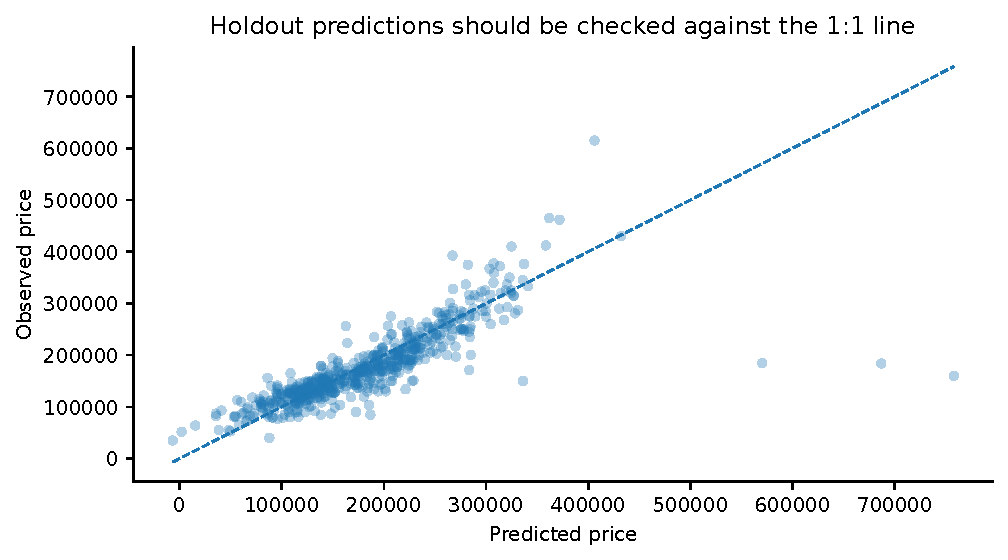
\includegraphics[width=0.66\linewidth]{figures_generated/regression_predicted_actual.pdf}
\end{utpfig}

\section{Linear-model assumptions are diagnostic questions}
For inference on coefficients, common assumptions include approximate linearity of the conditional mean, independent errors, constant error variance, and an error distribution suitable for the inferential approximation. For prediction, the practical emphasis shifts toward whether residual patterns indicate systematic failure on cases like those to be predicted.

\begin{utpfig}[Residual diagnostic]{A useful residual plot looks roughly patternless around zero. Curvature, funnels, clusters, or isolated points suggest model misspecification or heterogeneous error.}{fig:regression-residual-plot}
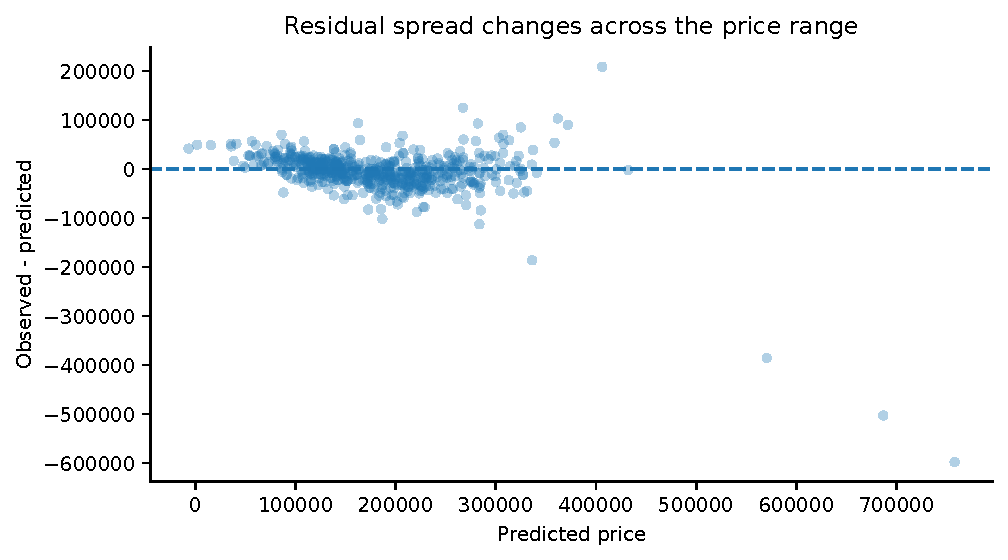
\includegraphics[width=0.79\linewidth]{figures_generated/regression_residual_plot.pdf}
\end{utpfig}

\section{Residuals reveal model failures}
Residual plots can expose curvature, non-constant variance, influential observations, or systematic subgroup errors. A single average metric can hide all of these.

\begin{pitfall}
Evaluating the model on the same rows used for fitting answers ``How well did the model remember the training data?'' rather than ``How well might it generalise?''
\end{pitfall}


\section{Underfitting and overfitting are both prediction problems}
A model that is too rigid can miss genuine structure; a model that is too flexible can fit sample-specific noise. Training error usually decreases with complexity, so model selection must rely on held-out or cross-validated performance.

\begin{utpfig}[Conceptual model-complexity curve]{Training error can keep improving while validation error eventually worsens. The useful level of complexity is determined by generalisation, not by the lowest training error.}{fig:regression-complexity}
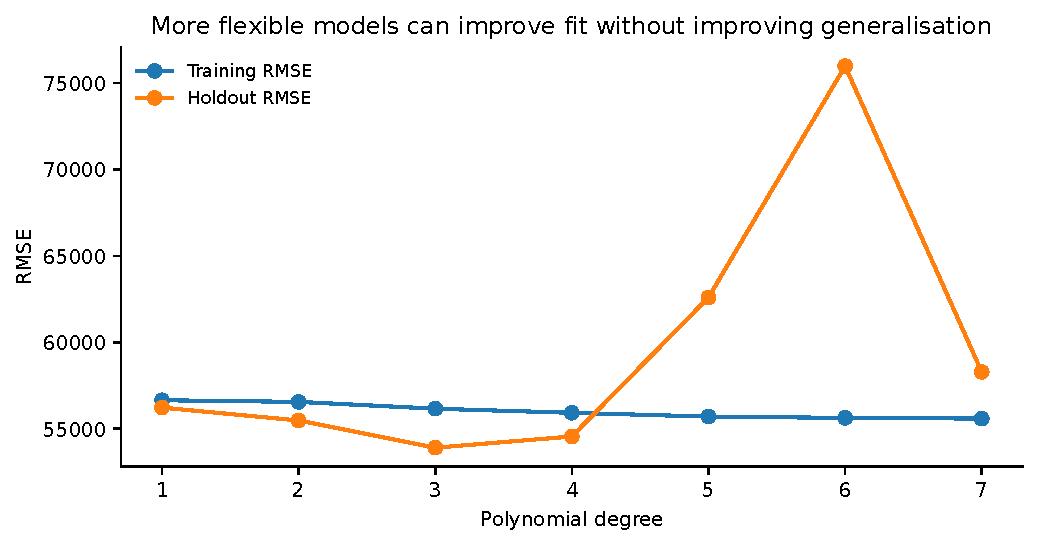
\includegraphics[width=0.80\linewidth]{figures_generated/regression_complexity.pdf}
\end{utpfig}


\section{Baselines make metrics meaningful}
Compare the regression against a simple baseline such as predicting the training-set mean for every case. A model that cannot improve on a naive baseline is not useful merely because it produced coefficients.

\begin{workedexample}
In Lab 7, alcohol is predicted from several other chemical measurements. The point is not to claim a production-ready chemistry model; it is to practise the complete supervised workflow: define target and features, split, fit, predict, evaluate, and inspect residuals.
\end{workedexample}

\begin{keyidea}
A predictive model is an empirical claim about unseen cases. Its credibility comes from validation data and transparent error analysis, not from how impressive the training summary looks.
\end{keyidea}

\begin{quickcheck}
\begin{enumerate}
  \item Why can a low training error be misleading?
  \item How do MAE and RMSE differ in their treatment of large errors?
  \item What can residuals reveal that \(R^2\) cannot?
  \item Why is a simple baseline useful?
\end{enumerate}
\end{quickcheck}

\section{Worked regression context: Ames Housing}

Ames Housing is deliberately more realistic than a small textbook regression table: 2,930 properties, 82 columns, mixed variable types, and substantial missingness in some attributes. The median sale price is \$160,000. Two strong raw associations are \texttt{Overall Qual} with sale price (correlation about 0.80) and above-ground living area with sale price (about 0.71).

\begin{utpfig}[Size, quality, and sale price]{Living area is positively related to sale price, but colour by overall quality reveals that similarly sized homes can occupy very different price ranges. Multivariable regression is useful precisely because one predictor rarely carries the whole structure.}{fig:reg-ames-area}
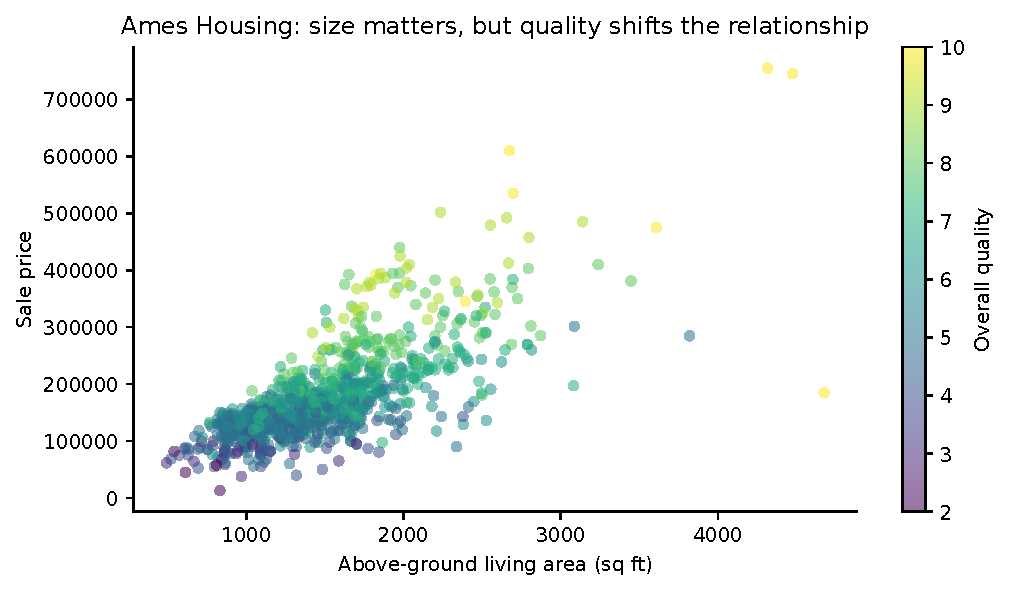
\includegraphics[width=0.86\linewidth]{figures_generated/regression_ames_area_price.pdf}
\end{utpfig}

A model can report a respectable $R^2$ and still fail in patterned ways. Diagnostic plots are therefore part of the model, not optional decoration.

\begin{utpfig}[Residual structure in a simple Ames model]{Residuals are observed minus fitted sale price. Curvature, changing spread, or extreme vertical deviations indicate information not captured by a simple linear specification.}{fig:reg-ames-residuals}
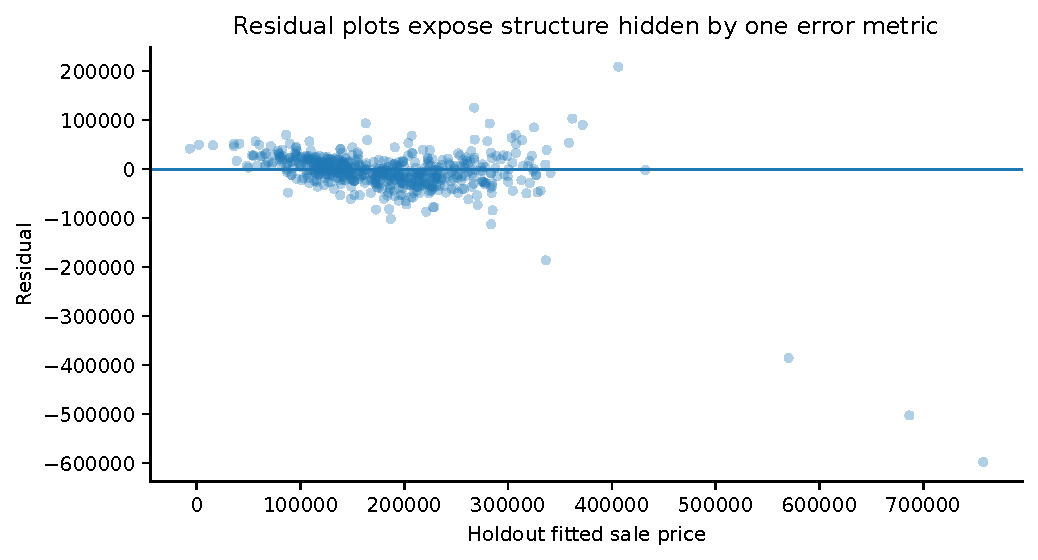
\includegraphics[width=0.82\linewidth]{figures_generated/regression_ames_residuals.pdf}
\end{utpfig}

Ames also introduces an important modelling decision: many categorical variables such as neighbourhood, building type, and exterior quality may be predictive, but including them requires careful encoding and stronger validation. The Lab 7 model starts with a small interpretable subset so students can diagnose the workflow before increasing complexity.


\section{Categorical predictors can carry structure that numeric summaries miss}

Ames Housing contains many categorical variables whose levels represent location, construction, or condition. Neighbourhood is a useful example because it produces clear price differences while also raising modelling questions about sparse levels, interpretation, and generalisation to future properties.

\begin{utpfig}[Neighbourhood groups have different price distributions]{The figure shows median sale price for neighbourhoods with at least 40 observations. The labels report group size so that a large median difference is not interpreted without knowing how much evidence supports it.}{fig:reg-ames-neighborhood}
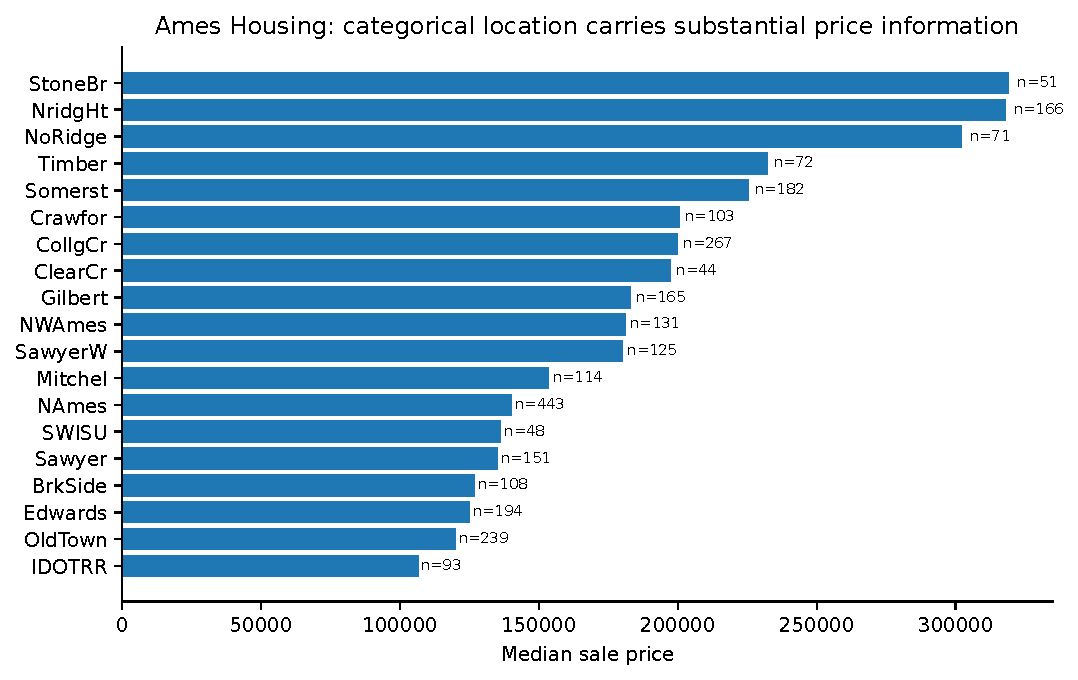
\includegraphics[width=0.88\linewidth]{figures_generated/regression_ames_neighborhood.pdf}
\end{utpfig}

A regression model cannot consume neighbourhood names as unordered text. Common approaches create indicator variables, combine rare levels, or use regularised encodings learned only from the training set. Whatever representation is chosen becomes part of the preprocessing pipeline and must therefore be reproduced exactly at prediction time.

\begin{pitfall}
Encoding a category using the target mean calculated from the full dataset is leakage. If target encoding is used, the encoding itself must be learned inside the training fold and applied to the corresponding validation fold without using its outcomes.
\end{pitfall}

